\section{Design Process or Methodology Overview
}

The vessel detection in this study has been performed using a multi-modal approach that incorporates radar and RGB images. Nevertheless, the radar images lack the clarity of optical images, which means we cannot determine the precision of this single modality; thus, we will reach a conclusion regarding the usefulness of radar images for this research outcome. RGB scenes provide valid results; however, their drawback is that they fail in specific conditions such as haze, overcast, or darkness.\\
Similarly, SAR images tend to be gritty and unclear. Thus, we employed five classifiers YOLO26-OBB~\cite{jocher2026ultralytics}, Faster R-CNN~\cite{7485869}, S2A-Net~\cite{han2021align}, OrientedFormer~\cite{zhao2024orientedformer} and Oriented R-CNN~\cite{xie2021oriented} to identify the ship using SAR and optical images, with feature extractors replicated for each source frame; the output layer remained unchanged, meaning any variations would indicate an issue with the classifier rather than with feature integration. Moreover, the dataset was meticulously utilized for model training to avoid both overfitting  and all five classifiers were trained on the same dataset to maintain control over the experiment.\\

Numerous targets were created, primarily to maintain uniformity in the aggregation unit across all architectures, where both radar and optical illustrations served as the source frame. Secondly, for the training aspect, we must ensure that data leakage does not occur, as it would lead to memorization of predictions rather than genuinely understanding the answers.Additionally, we need to evaluate performance on a specific part of dataset to assess how well the architecture functions, thirdly, it is essential to assess whether the radar enhances to image classification by comparing the outcomes:one result containing only radar values, another without any values, and finally a falsified radar image to evaluate the model's training effectiveness. Fourthly, identify ships of various sizes and assess the strength, weakness, clarity, brightness, or darkness of the image, noting how the outcome varies accordingly. Ultimately, for all architectures, we achieved 99 percent accuracy with mAP50, which is a slightly misleading outcome for the classifiers;however, a performance comparison was conducted when mAP50:95 was considered.


\\
\begin{figure}[htbp]
    \centering
    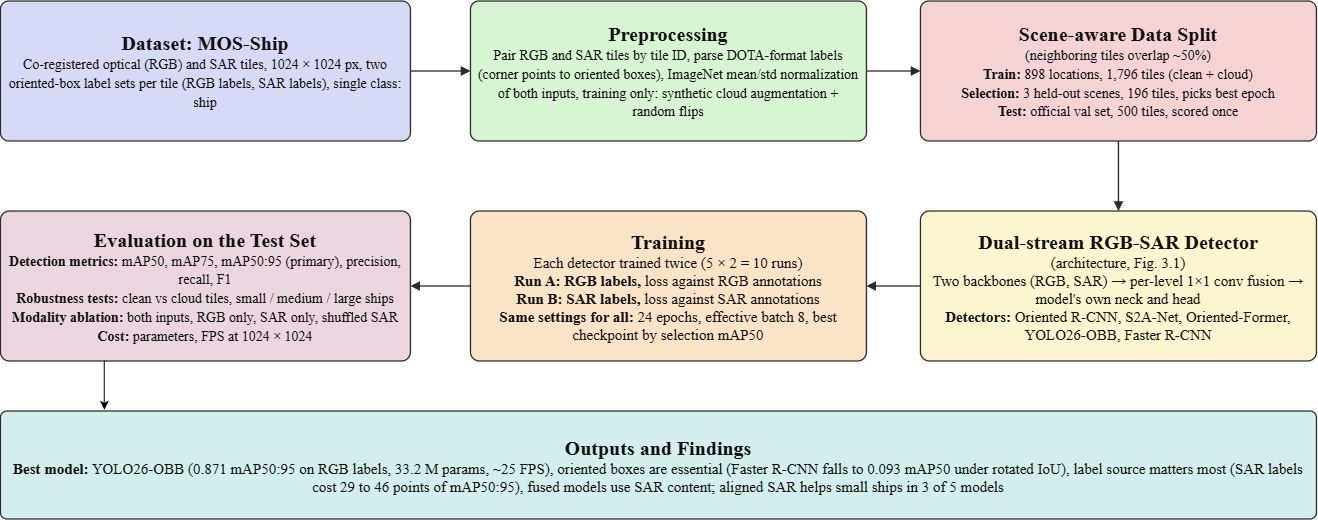
\includegraphics[width=1\textwidth]{images/p2_methodology_flowchar.png}
    \caption{Methodology flowchart of the proposed system.}
    \label{fig:methodology_flowchart}
\end{figure}
\FloatBarrier

\\


\subsection{Design Constraints}\\

\textbf{Computational Efficiency (Hardware-Constrained Training):}All models that we have used in this study needs to be trained and perform the inference at 1024×1024 resolution within the limits of a single 8 GB consumer-grade GPU (RTX 3070 / RTX 3070 Ti), because this reflects the actual compute budget that is available for the project. This constraint resulted in shaping the training configuration which is an effective batch size of 8 that was achieved through the gradient accumulation (2×4 for most detectors, 1×8 for OrientedFormer~\cite{zhao2024orientedformer}), and mixed-precision training (fp16/bf16) was required to fit within available VRAM. \\

\textbf{Ship Orientation and Dense Port Scenes:}Ships can appear at arbitrary angles relative to the image frame, and a simple axis-aligned bounding box fails to correctly capture the true bounding of an elongated ship which is particularly problematic if multiple ships are docked closely together. In such cases, the individual horizontal boxes might block each other. That is why ,we have decided to use oriented bounding boxes as the primary target of detection for all applicable models in this study. A quick inspection of the validation set suggests this is a real issue: tiles contain on average 2.2 ships each (up to a maximum of 12), 36 of 250 tiles have 5 or more vessels, and approximately 23 percent of ships have a horizontal-box IoU overlap of more than 0.1 with a neighboring vessel (though only a small number (five) of ship pairs have IoU overlap of more than 0.5). That is mainly why we have chosen oriented detection as a design choice.\\

\textbf{Multi-Modal Annotation and Representation Inconsistency:
}Among the two main problems, firstly the SAR and RGB images can have different ground-truth boxes for the same ship because the two sensors capture the scene differently(different box location/shape for the same vessel for different channels/modalities due to sensor geometry). And secondly, It is mentioned in the description of the dataset that the SAR channel data is single-channel 32-bit float for it to preserve the full backscatter dynamic range, whereas in the SAR images we have only 8-bit 3-channel visualizations, with no availability of the original floating-point products.\\

\newpage
\textbf{SAR-Specific Degradation (Sea Clutter and Speckle Noise) :} SAR images are prone to speckle noise and sea clutter, which makes the ship detection difficult. These can create a false-alarm and confuse the subject which is one of the relevant concerns of our work.  However, in this  phase we have only applied ImageNet-style normalization to the SAR input in the  preprocessing pipeline  that does not remove speckle noise. This constraint remains an open item for future work to solve.\\

\textbf{Optical Occlusion via Cloud Cover:} Even though our RGB-SAR fusion approach is designed in this way so that SAR can come in handy when an optical image is affected by clouds and gives inaccurate answers but still, our current results doesn't show much significant difference between clean and cloud-affected images when SAR is not used (0.967 vs. 0.971). Therefore,  we still can’t confidently claim that SAR clearly improves cloud-robustness, which leaves us room for further improvement in the upcoming  research. \\

\textbf{Class and Scale Imbalance :} Our dataset contains more medium sized ships than the small ones, so the ships that are around 20 meters or less are usually tough to detect accurately using an oriented detection model. Hence, detecting the small ships precisely remains as a constraint that our current work has not been able to resolve yet.\\

\subsection{Strategy and Research Phases
}The research is conducted in six phases, each of which answers a particular question and the results of each phase inform the next phase of research.\\

\textbf{Phase 1: Data Preparation and Evaluation Protocol}\\
In the first phase, a stable and reproducible experimental environment is prepared.The preprocessed RGB and SAR data, data pipeline and evaluation procedure are the same for all models. The overlap between neighbouring tiles is approximately 50 percent, which means that if a tile-level split is done randomly, there may be information leakage between training and evaluation data. In order to minimize this risk, three whole scenes are kept as a scene-based selection split. This split allows for a dedicated scene-level set to monitor model performance and choose the optimal checkpoint, and also keeps the checkpoint-selection process away from the official evaluation data. The official validation split is reserved as the final test set and is only assessed after model selection. This makes it easier to compare the detection models.\\

\textbf{Phase 2: Baseline Detector Comparison}\\
The second phase tests various detection architectures with multimodal (RGB and SAR) inputs. Five detectors are implemented, including Oriented R-CNN~\cite{xie2021oriented}, S²A-Net~\cite{han2021align}, OrientedFormer~\cite{zhao2024orientedformer}, YOLO26-OBB~\cite{jocher2026ultralytics}, and Faster R-CNN~\cite{7485869}, all of which are based on the same dual-stream fusion idea. The models are first trained with RGB ground truth. Because mAP50 is very high across the models, mAP50:95 is given more weight when comparing the detection performance of the models, especially to assess the quality and localization accuracy of the predicted bounding boxes.\\

\textbf{Phase 3: Test time modality Ablation}\\
The third phase explores the role of each modality in the multimodal detectors during test time. The trained models are tested with RGB-only, SAR-only, RGB + SAR and shuffled-SAR inputs. Results indicate that SAR can be used as a valuable supplementary information if the right SAR image is applied, and an incorrect SAR image results in a significant performance degradation. But if RGB ground truth is used, the models that have been removed RGB perform close to zero, indicating that the initial fusion models are heavily dependent on the RGB stream.
\\

\textbf{Phase 4: SAR Ground Truth Evaluation}\\
The fourth phase explores the possibility that this high reliance on RGB is partly due to the selection of ground truth. MOS-Ship also offers two distinct sets of RGB and SAR annotations, which are not the same, and the models are retrained on SAR ground truth and evaluated with the same modality-ablation procedure~\cite{you2026multi}. In this case, SAR-only detection works well, and the results are significantly better than the near zero results obtained when SAR was evaluated against RGB ground truth. This indicates that the earlier failure (SAR only) does not mean that SAR is incapable of detecting ships and that the source of annotation has a significant impact on the measured modality performance. In the experiments, however, SAR is still the weaker stand-alone modality, with its performance still being lower than the combined RGB + SAR performance than the RGB-only performance under RGB ground truth.
\\

\textbf{Phase 5: Balanced Multimodal Training and Robustness}\\
The fifth phase is the next step of the research and will be based on the results of the modality-ablation and SAR-ground-truth experiments. The goal is to lessen the reliance on a single modality and enhance the role of both RGB and SAR in the fusion model. Future experiments will involve modality dropout, experiments with a reference model using only RGB data, experiments using only SAR data, and experiments with more severe optical degradation (heavier cloud conditions, optical blackout). These experiments will test the fusion model to see if it can continue to reliably detect ships when one modality is partially or completely unreliable.\\

\textbf{Phase 6: Future Vessel Tracking}\\
The sixth phase is a future extension of the research.Once a stable multimodal ship detection system is developed, temporal information can be added to solve the problem of vessel trajectory tracking and reconstruction. This stage will explore the potential of associating detections from multiple observations over time and the use of trajectory information to estimate a vessel's movement when observations and/or communication signals are not available.\\


\section{Preliminary Design or Design (Model) Specification} 
Five object detectors :Oriented R-CNN\cite{xie2021oriented}, S2A-Net~\cite{han2021align}, OrientedFormer~\cite{zhao2024orientedformer}, YOLO26-OBB~\cite{jocher2026ultralytics} and Faster R-CNN~\cite{7485869}. Four of them predict oriented bounding boxes whereas Faster R-CNN~\cite{7485869} predicts horizontal boxes. These five models comprises one stage, two stage, transformer based and real time based detectors. They were originally designed for a single RGB image and thus the same dual stream RGB-SAR front end was given to each model as shown in figure: \ref{fig:dual_stream_design}\\

\subsection{Shared Dual-Stream RGB-SAR Design
}
\begin{figure}[htbp]
    \centering
    \includegraphics[width=0.6\textwidth]{dual_stream_design.png}
    \caption{Dual-stream architecture of the proposed system.}
    \label{fig:dual_stream_design}
  
\end{figure}
% \FloatBarrier


Each model uses two distinct backbones; one processes the RGB tiles and other processes SAR tiles. At each feature level, feature map from both backbones are concatenated and then applied to a 1x1 convolution\\
\begin{equation}
F_l = \operatorname{Conv}_{1\times1}
\left(
\left[ F_l^{RGB} \,;\, F_l^{SAR} \right]
\right)
\label{eq:rgb_sar_feature_fusion}
\end{equation}

where $F_l^{RGB}$ and $F_l^{SAR}$ are the stream features at level $l$.
The fusion initially starts with equal weight to both modalities but eventually
learns the weight of each modality and updates and adjusts the $1\times1$
convolution weights during training. The resulting features are then fed into
the feature pyramid and head of the original detector. As a result, only
feature extraction is altered without changing the detection process.

Feature level fusion was chosen because it accommodates RGB and SAR without altering the pretrained backbone layer. Simply adding SAR or RGB in channel level fusion would affect the first layer, while merging the bounding box at the end would limit SAR's ability to improve localization of ship that are partly visible or hardly visible in the RGB image.\\

\textbf{Ground truth reference: }Although MOS-Ship gives separate RGB and SAR labels, they show noticeable differences~\cite{you2026multi}. The centers of the matched boxes The matched RGB and SAR bounding boxes showed limited alignment where only 44\% of the matched boxes reached an IoU of at least 0.5. Only 19 pixel distances at the median between the center of the bounding boxes suggest that the differences mainly comes from box shape and size rather than its location. Therefore, RGB labels are used as consistent references for both training and testing whereas SAR labels are provided as additional input. All models were later retrained using SAR label as well to evaluate the effect of label choice.
\\

\textbf{Box format:}All oriented models follow the ``le90'' convention for bounding boxes.
$(x, y, w, h, \theta)$ is the base box form, where $(x, y)$ is the centre,
$w \geq h$, and $\theta \in [-\pi/2, \pi/2)$.

For a fair evaluation, the box coder, data loader, and evaluation codes are
also shared. As a result, the differences in scores will be fostered by the
models and not by the pipeline.\\

\subsection{Baseline Detector Architectures}\\

\textbf{1. Oriented R-CNN}

\\

\begin{figure}[htbp]
    \centering
    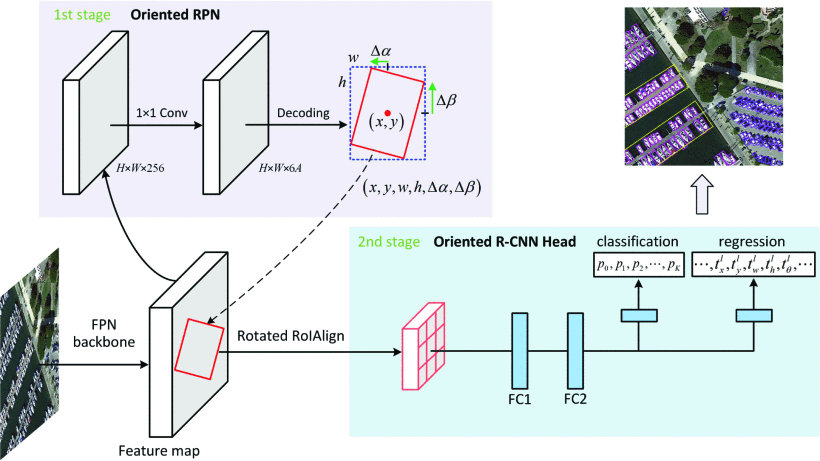
\includegraphics[width=0.6\textwidth]{images/model_diagram/oriented-rcnn.png}
    \caption{Architecture of the Oriented R-CNN model~\cite{xie2021oriented}.}
    \label{fig:oriented_rcnn}
\end{figure}

\FloatBarrier
\\

ORCNN uses a feature extractor named ResNet-50 which captures feature maps C2,C3,C4,C5 these are then fused together using FPN to produce hierarchical feature representation of P2,P3,P4,P5,P6~\cite{xie2021oriented} .Then Oriented RCNN applies these features and oriented proposals are constructed which estimates six spatial information (x,y,w,h,Δx,Δy) relative to horizontal reference boxes through midpoint-based representation . The proposed regions are then fed into RoI feature extraction to extract features from the regions, and the detection head is used to classify the object and adjust the position of the region. Throughout end-to-end training, the model concurrently learns object localization, classification, oriented region suggestions, and feature representations.\\

\textbf{2. S2Anet}\\

\begin{figure}[htbp]
    \centering
    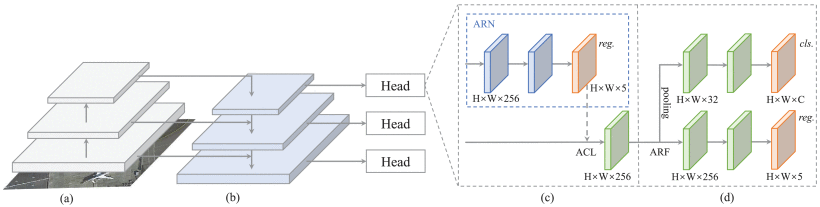
\includegraphics[width=0.8\textwidth]{images/model_diagram/s2a-net.png}
    \caption{Architecture of the S2A-Net model~\cite{han2021align}.}
    \label{fig:s2a_net}
\end{figure}

\FloatBarrier
S2Anet~\cite{han2021align} functions as a one-stage classifier.The process consists of receiving two images as input, replicating the backbone, merging the feature maps at every level, and utilizing a single FPN to manage the scale.Then,it rotates the horizontal anchor box employing FAM, and with the rotated anchor, it examines the sampling point through alignment convolution and aligns with the slanted image. Subsequently, ODM employs a filter to generate eight variations of it, which are fundamentally used to accurately classify the ship no matter the direction it is facing and to identify the rotated bounding box regression. Moreover, four losses are calculated, a bounding box is generated, and similar boxes are eliminated. The design is a one-stage detection framework that includes a Feature Alignment Module (FAM) and an Oriented Detection Module (ODM). The main innovation involves utilizing alignment convolution to adjust the sample point and employing FAM to rotate the horizontal normal anchor boxes for viewing the estimated slanted object. The design principle states that for the inclined object, we utilize ODM for bounding box classification and regression following the application of FAM to adjust the anchor boxes for spatial alignment. The main characteristic is that various filters are used for ships oriented in different directions, and pooling is applied to identify the ship regardless of its facing. In both FAM and ODM, focal loss and smooth L1 are utilized, resulting in a total loss composed of four components. ARN understands how to adjust horizontal anchors into oriented anchors, while ACL determines the appropriate offset to align samples with the angle of the anchors. The decoupling of ODM resolves the conflict between classification and regression.Additionally, the oriented boxes are interpreted and refined at inference using rotated NMS. The paper does not report the parameter count or FLOPs for S2A-Net (Liu et al.,2023)~\cite{han2021align}.
\\

\newpage
\textbf{3. OrientedFromer}
\\

\begin{figure}[htbp]
    \centering
    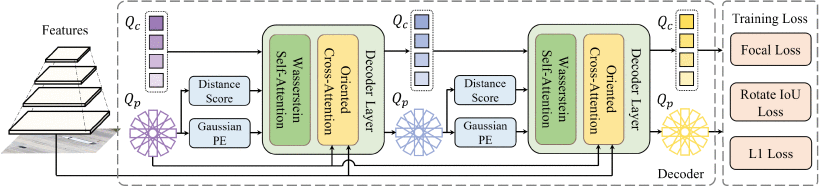
\includegraphics[width=1\textwidth]{images/model_diagram/oriented-former.png}
    \caption{Architecture of the OrientedFormer model~\cite{zhao2024orientedformer}.}
    \label{fig:oriented_former}
\end{figure}

\FloatBarrier
OrientedFormer~\cite{zhao2024orientedformer} is a Transformer-based detector designed specifically to recognize objects that appear in orientations. The model uses a ResNet-50 backbone to extract features at scales. It picks four feature layers from this backbone to collect information from levels of detail. These features are then passed through a channel mapper. Sent directly to the Transformer decoder. There is no need for a Transformer encoder in this setup.
The decoder works with object queries that are divided into two parts: content queries and positional queries. The positional queries tell the model where the object is located, how big it is and what direction it faces. To represent the oriented bounding box the model uses Gaussian Positional Encoding. This method treats the bounding box as a two- Gaussian distribution, which helps the model learn position, size and angle all at once.
Wasserstein Self-Attention improves the way the model focuses on parts of the image. It uses the relationships between the Gaussian representations of different queries to make attention more accurate. Oriented Cross-Attention changes how the model samples features. It adjusts the sampling points based on the expected orientation of the object so the features it picks match the direction of the object closely.
After processing the decoder predicts the class of the object and the oriented bounding box for each query. During training the model uses one-to-one matching to link predictions to real objects. It uses Loss for classification, L1 loss for bounding box regression and Rotated IoU loss to better handle the orientation of the boxes. These losses are applied at each decoder layer allowing the model to learn classification, localization and orientation simultaneously.
The ResNet-50 version of OrientedFormer~\cite{zhao2024orientedformer} has around 44 million parameters. Requires about 529 GFLOPs. It runs at a speed of 11.4 frames per second, on the DOTA-v1.0 dataset.
\\

\textbf{4. YOLO26-OBB}
\\

\begin{figure}[htbp]
    \centering
    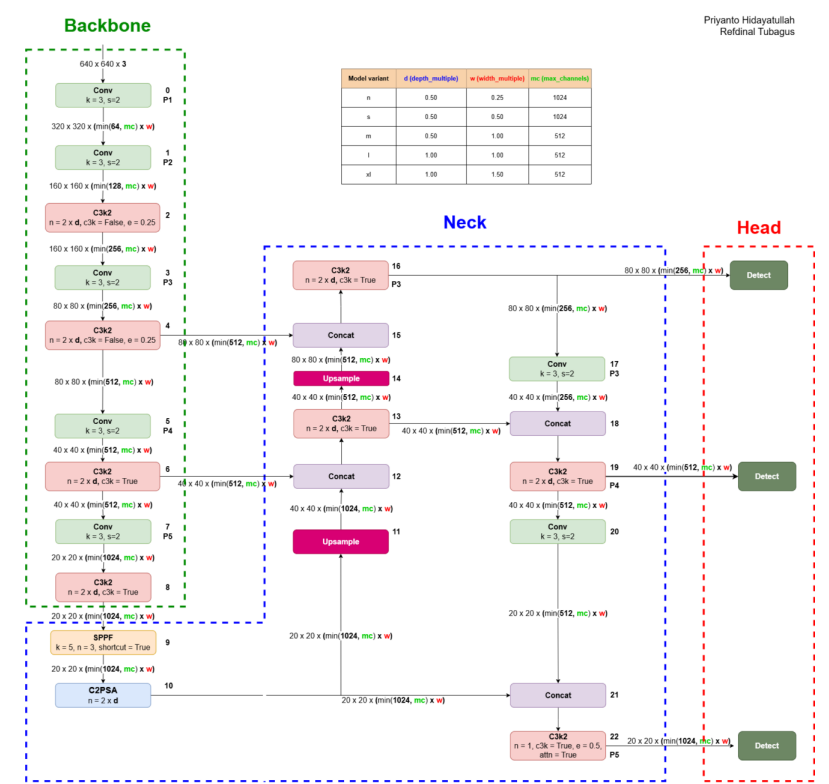
\includegraphics[width=0.7\textwidth]{images/model_diagram/yolo26.png}
    \caption{Architecture of the YOLO26 model~\cite{Hidayatullah2026YOLO26AC}.}
    \label{fig:yolo26}
\end{figure}
\FloatBarrier

YOLO26-OBB~\cite{jocher2026ultralytics} is a one stage, anchor free and NMS free model for detecting rotated objects in aerial images. It was released by Ultralytics and later described in their official paper~\cite{jocher2026ultralytics}. Before that paper came out, Hidayatullah and Tubagus~\cite{Hidayatullah2026YOLO26AC} worked out its architecture from the source code, which is where Figure~\ref{fig:yolo26} comes from. The model comes in five sizes: n (nano), s (small), m (medium), l (large) and x (extra large). The backbone has 11 layers built from Conv, C3k2, SPPF and C2PSA blocks. Layers 4, 6 and 10 give the P3, P4 and P5 feature maps at strides 8, 16 and 32. A PAN-FPN neck then mixes these maps through top-down and bottom-up paths~\cite{Hidayatullah2026YOLO26AC}. The OBB head predicts the angle directly, without a sigmoid. Boxes use a long-edge form, where the longer side is the width and the angle lies in [-45°, 135°). The head has two branches, one-to-many and one-to-one. Both are trained, but only the one-to-one branch is used at inference. It keeps the top 300 boxes, so no NMS is needed. YOLO26 also drops DFL and regresses box edges directly with an L1 loss~\cite{jocher2026ultralytics}. The box loss combines ProbIoU with this L1 term, and the class loss is BCE. An extra angle loss gives more weight to nearly square objects, because the IoU loss barely changes with their angle. Labels are assigned with a task aligned assigner. The one-to-many branch takes up to 10 candidates per ground-truth box. The one-to-one branch takes 7 and keeps only the best one. STAL enlarges box sides smaller than 16 pixels to 16 pixels during this selection, so tiny ships still get positive samples. Progressive loss moves the branch weights from 0.8 (one-to-many) and 0.2 (one-to-one) to 0.1 and 0.9 over training~\cite{jocher2026ultralytics}. In our thesis, we build a dual-stream version with two YOLO26-m backbones, one for RGB and one for SAR. Their P3, P4 and P5 maps are fused by a 1×1 convolution. This convolution starts as the mean of the two streams. The fused maps then go through the YOLO26 neck and OBB head. Both backbones, the neck and the head start from Ultralytics' DOTAv1~\cite{xia2018dota} OBB checkpoint, and the class weights are copied from its ship class. The model has 33.15 million parameters at inference, after the one-to-many branch is removed. We use Ultralytics only for the model, loss and EMA code, not for its trainer or data loader. We train with AdamW instead of the MuSGD optimizer that Ultralytics~\cite{jocher2026ultralytics} uses for DOTA. Augmentation is limited to random horizontal, vertical and diagonal flips. Backbone layers 0 to 2 are frozen in both streams, and training runs in bf16 mixed precision. EMA weights are used for validation and for picking the best checkpoint. The RGB annotations serve as ground truth. Oriented boxes let the model fit ships at any angle much more tightly than horizontal boxes.\\

\textbf{5. Faster R-CNN}
\\

\begin{figure}[htbp]
    \centering
    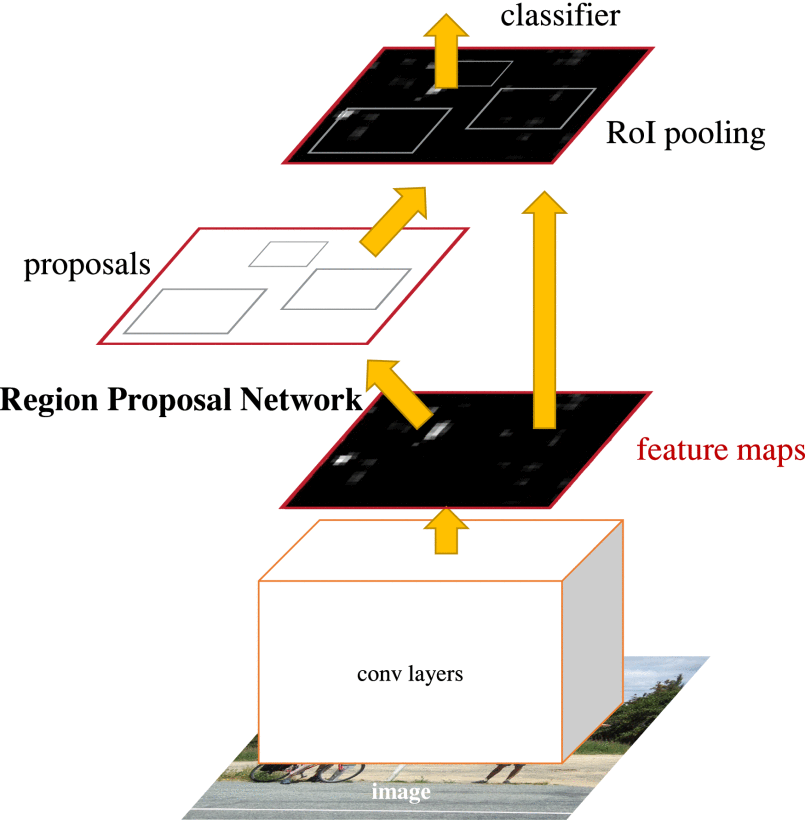
\includegraphics[width=0.5\textwidth]{images/model_diagram/faster-rcnn.png}
    \caption{Architecture of the Faster R-CNN model~\cite{7485869}.}
    \label{fig:faster_rcnn}
\end{figure}

\FloatBarrier
\\
The model includes parallel backbones that accept 2 input images from SAR and optical sources, generating feature maps that are produced and combined at different layers. The RPN indicates possible locations for the object, after which we apply RoIAlign to enhance features, and then classify our ship along with the bounding box using faster R-CNN~\cite{7485869}. The main innovation utilizes a Region Proposal Network to detect possible objects and then performs classification and bounding box refinement. The design philosophy first identifies possible ship locations, then examines each area more closely to ascertain if it is a ship and adjusts its bounding box accordingly. The conventional single-stream ResNet-50 Faster R-CNN setup comprises approximately 41.35 million parameters and incurs a computational cost of about 134.52 GFLOPs.

\subsection{Comparative Analysis}

\\
\newlength{\tw}  % define once only; delete this line if you paste a second table that also uses \tw

\begin{table}[htbp]
\centering
\footnotesize
\renewcommand{\arraystretch}{1.5}
\setlength{\tabcolsep}{4pt}
\setlength{\tw}{\dimexpr\textwidth-16\tabcolsep-9\arrayrulewidth\relax}

\begin{tabular}{
|>{\raggedright\arraybackslash}p{0.19\tw}
|>{\raggedright\arraybackslash}p{0.15\tw}
|>{\raggedright\arraybackslash}p{0.06\tw}
|>{\raggedright\arraybackslash}p{0.11\tw}
|>{\raggedright\arraybackslash}p{0.09\tw}
|>{\raggedright\arraybackslash}p{0.09\tw}
|>{\raggedright\arraybackslash}p{0.12\tw}
|>{\raggedright\arraybackslash}p{0.19\tw}|
}
\hline
\rowcolor{gray!20}
\textbf{Model} &
\textbf{Type} &
\textbf{Box} &
\textbf{DOTA-v1.0~\cite{xia2018dota}mAP50 (\%)} &
\textbf{DOTA ship~\cite{xia2018dota} AP (\%)} &
\textbf{HRSC 2016 mAP (\%)} &
\textbf{Speed} &
\textbf{Source} \\
\hline

Faster R-CNN (FR-H) &
Two-stage &
HBB &
60.46* &
50.04* &
- &
- &
Xia et al., 2018~\cite{xia2018dota} \\
\hline

Faster R-CNN (FR-O) &
Two-stage &
OBB &
54.13 &
37.16 &
- &
- &
Xia et al., 2018~\cite{7485869} \\
\hline

Oriented R-CNN &
Two-stage &
OBB &
75.87 &
88.20 &
96.50 &
15.1 FPS &
Xie et al., 2021~\cite{xie2021oriented} \\
\hline

S2A-Net &
One-stage &
OBB &
74.12 &
87.25 &
95.01$^{\dagger}$ &
16.0 FPS &
Han et al., 2021~\cite{han2021align} \\
\hline

OrientedFormer &
Transformer, end to end &
OBB &
75.37 &
88.29 &
96.48 &
11.4 FPS &
Zhao et al., 2024~\cite{zhao2024orientedformer} \\
\hline

YOLO26-OBB &
One-stage, end to end &
OBB &
81.0$^{\ddagger}$ &
- &
- &
10.2 ms (T4, TensorRT) &
Jocher et al., 2026~\cite{jocher2026ultralytics} \\
\hline
\end{tabular}

\caption{Literature-based performance of the selected detectors}
\label{tab:literature_performance}
\end{table}

\\
Table~\ref{tab:literature_performance} shows the reported performance of the selected detectors. Three points have guided our decisions here:\\
Firstly, oriented boxes are important for ship detection. In DOTA~\cite{xia2018dota},the early oriented Faster R-CNN baseline got 37.16\% AP for ships,whereas the three oriented detectors achieved around 87\%-88\% AP. Even though newer backbones and training methods could contribute to this result,horizontal boxes can include a large amount of sea around diagonal ships and may result in overlapping with the nearby ships,which is why using oriented boxes is just as crucial.Therefore,four out of our five selected models use oriented boxes. \\
Furthermore, among the models,there is no clear single best model. Oriented R-CNN~\cite{xie2021oriented}, S2A-Net~\cite{han2021align} and OrientedFormer~\cite{zhao2024orientedformer} have a similar performance which are within about 1.8 points on DOTA~\cite{xia2018dota} and 1.5 points on HRSC2016. So, by taking one of each,we can check if the RGB-SAR fusion performs the same across different detector family models.\\

Lastly, fast detection is crucial in real-time ship monitoring and that’s why YOLO26-OBB~\cite{jocher2026ultralytics} is designed for faster real-time object detection which can pinpoint the oriented bounding boxes without using NMS. This model allows us to compare heavier models against a faster,more deployment focused detector,and see how it performs. 
\\

\section{Data Collection 
} Our research uses the MOS-dataset which was introduced by You et al.~\cite{you2026multi} in the paper "A Multi-Modal Approach for Robust Oriented Ship Detection: Dataset and Methodology". \\
We collected the dataset from the authors' official GitHub repository, which hosts the dataset download (via Baidu Netdisk) along with the paper's reference implementation. The main repository of the research does include an Apache License 2.0 file, however, the README file does not come with a separate license statement that is specific to the satellite imagery, hence we have cited the dataset to the original authors and repository throughout our whole work.
\\

\subsection{Dataset Characteristics} 
In the dataset, the MOS-Ship pairs come in co-registered optical (RGB) and Synthetic Aperture Radar (SAR) imagery form, with oriented bounding-box annotations~\cite{you2026multi}. The dataset comes with a  single object class, named "ship". Each scene is given as a pre-tiled 1024×1024 patch, along with a corresponding SAR patch and two separate DOTA-format~\cite{xia2018dota} annotation files. A sample tile is shown in Figure~\ref{fig:mosship_sample}.

\begin{figure}[htbp]
    \centering
    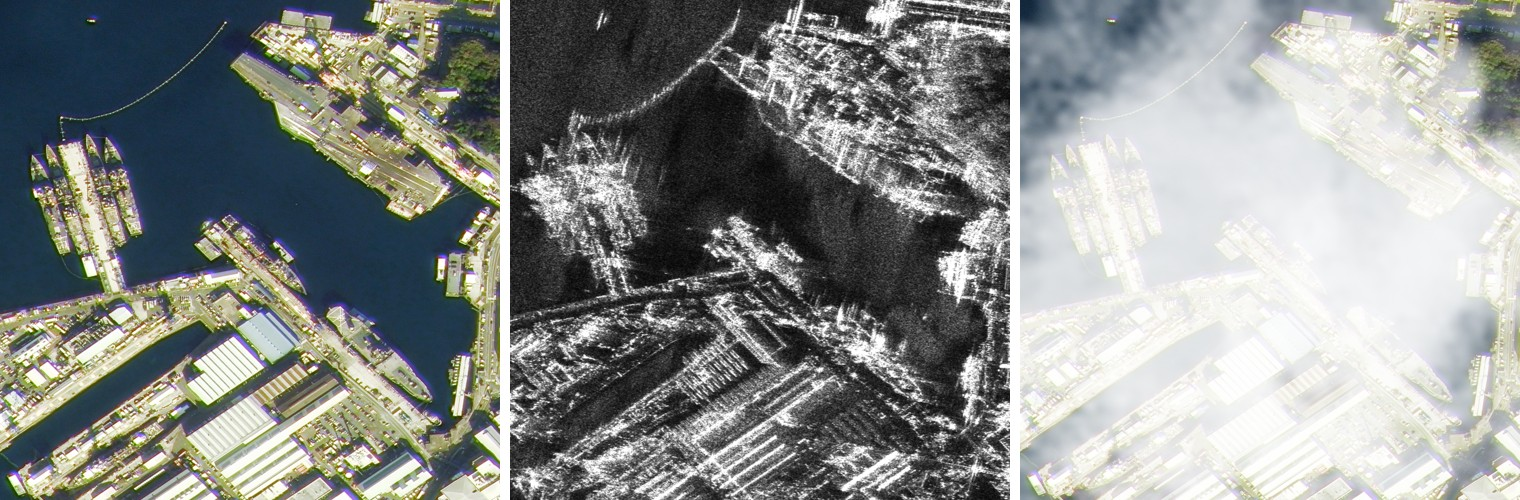
\includegraphics[width=\textwidth]{images/dataset_image/dataset-image-demo.jpg}
    \caption[Sample tile from the MOS-Ship dataset]{Sample tile from the
MOS-Ship dataset~\cite{you2026multi}. Left to right: optical RGB image,
co-registered SAR image of the same area, and optical image with
synthetic cloud cover.}
    \label{fig:mosship_sample}
\end{figure}

The publicly released dataset provides only the finalized, tiled product of the authors' original data-curation pipeline.In the paper, the large-scale optical and SAR data that have been used for LightGlue-based feature matching and RANSAC affine co-registration step have not been released. Which is why, the 1024×1024 co-registered tiles are only the publicly available ones. Since the released dataset already contains this pre-processing,thus,we have not performed the same preprocessing again on the dataset.\\

\subsection{Data Transformation and Augmentation}

\\
\begin{figure}[htbp]
    \centering
    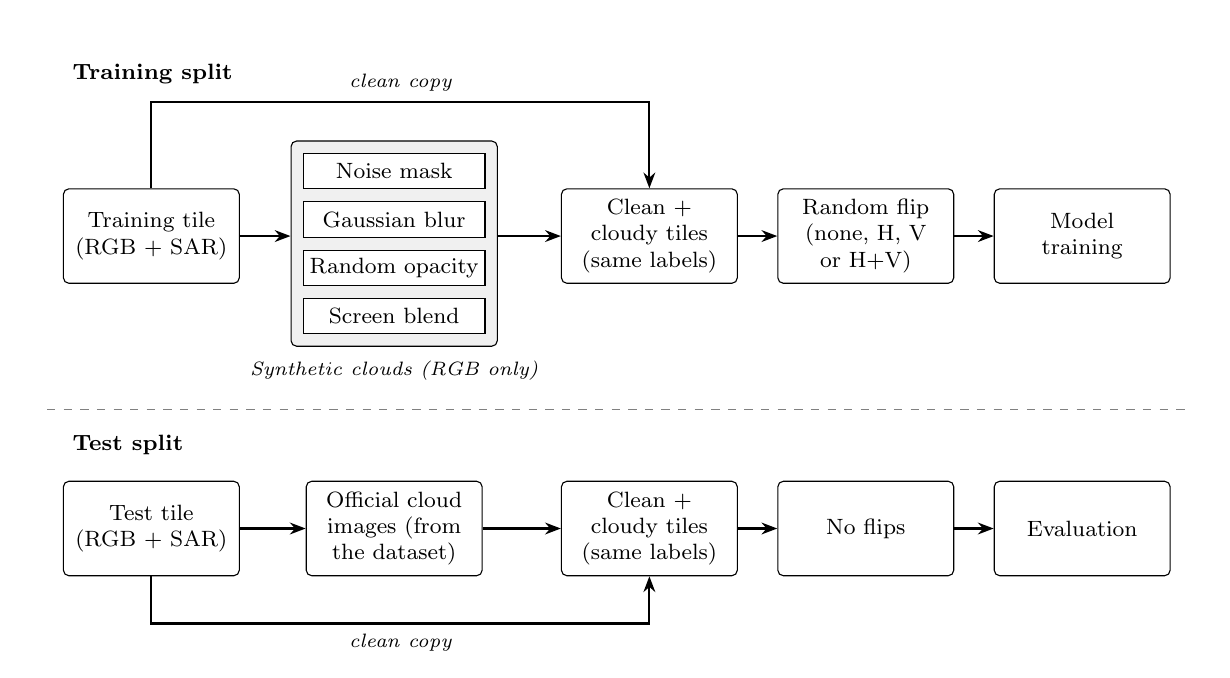
\includegraphics[width=\textwidth]{images/data_transformation.png}
    \caption{Data transformation process}
    \label{fig:data_transformation}
\end{figure}
\\
The MOS-dataset's official cloud augmentation was previously retained as part of the training pipeline~\cite{you2026multi}. To add the synthetic clouds in the training split, irregular noise-based cloud masks, randomized opacity ranging from 0.6 to 1.0, Gaussian blur, and screen blending programmatic systems have been used. And as for the validation and test splits, we have used the dataset's own pre-generated cloud-augmented images. The same ground-truth annotations have been maintained for both clean and cloud-augmented images. Lastly, along with cloud augmentation, random horizontal, vertical, and diagonal flips have also been applied during model training to improve the model's potential, so that it can generalize into different image orientations.

\subsection{Summary of Preprocessed Data }We have built a preprocessing pipeline which converts the dataset so that it can be used directly by the models. The pipeline includes the following steps:
\\

\textbf{1. Pairing :} In this step, the  RGB and SAR image were matched using their tile identifiers where the pipeline auto-detectects the dataset's two distinct folder layouts used for the  training and validation sets.\\

\textbf{2. Annotation parsing :} The DOTA-format~\cite{xia2018dota} label files  were examined to extract each ship's four corner coordinates(bounding-box annotations),object category, and a trailing identifier field.
\\

\textbf{3. Normalization :} The pixel values of the RGB and SAR images were normalised by using ImageNet mean and standard deviation .\\

\textbf{4. Output formatting :} Finally , we saved the normalized images and the parsed annotations in separate files and created another file linking each sample with its RGB and SAR images.
\\

\subsection{Train / Selection / Test Organization}

The MOS-Ship dataset comes with an official train and validation split~\cite{you2026multi}. In the dataset, tiles are 1024 pixels in size and these are generated every 500 pixels, which results in the neighboring tiles to overlap by about half of their area.Therefore,randomly splitting the tiles into training and validation could result in potential data leakage as the portion of the tile present in the validation test could also be present in the training set due to the overlap.To avoid such a scenario, we have separated three entire scenes from the training split and created a new ‘selection set’ which is used to choose the best model checkpoint during model training. We have kept the official validation split unchanged and used it as the final test set to evaluate the final model performance. Table~\ref{tab:final_data_split} shows the final data split.
\\

\begin{table}[htbp]
\centering
\small
\renewcommand{\arraystretch}{1.3}

\begin{tabular}{
|>{\raggedright\arraybackslash}p{0.25\textwidth}
|>{\centering\arraybackslash}p{0.18\textwidth}
|>{\centering\arraybackslash}p{0.16\textwidth}
|>{\centering\arraybackslash}p{0.16\textwidth}
|>{\centering\arraybackslash}p{0.15\textwidth}|
}
\hline

\rowcolor{gray!20}
\textbf{Split} &
\textbf{Unique tile locations} &
\textbf{Clean tiles} &
\textbf{Cloud tiles} &
\textbf{Total rows} \\
\hline

Train &
898 &
898 &
898 &
1796 \\
\hline

Selection &
98 &
98 &
98 &
196 \\
\hline

Test (official val) &
250 &
250 &
250 (official) &
500 \\
\hline

\end{tabular}
\caption{Final data split}
\label{tab:final_data_split}

\end{table}



\subsubsection{{Final Dataset Statistics}}
Based on the size of the bounding box, the ships were divided into three size categories following the thresholds given in the source paper: small ($< 64^2$), medium ($64^2$--$128^2$), and large ($> 128^2$). We have calculated the counts from the RGB annotations of the clean and non-cloud images because the clean images also contain its corresponding cloud-augmented copy with the same annotations .Thus, the number of instances gets doubled when both versions are included resulting in 4,034 ship instances in training and 1,098  ship instances in testing. Table~\ref{tab:ship_scale_distribution} shows the number of ships in each size category.
\\

\begin{table}[htbp]
\centering


\small
\renewcommand{\arraystretch}{1.3}

\begin{tabular}{
|>{\raggedright\arraybackslash}p{0.30\textwidth}
|>{\centering\arraybackslash}p{0.14\textwidth}
|>{\centering\arraybackslash}p{0.14\textwidth}
|>{\centering\arraybackslash}p{0.14\textwidth}
|>{\centering\arraybackslash}p{0.14\textwidth}|
}
\hline

\rowcolor{gray!20}
\textbf{Split} &
\textbf{Small} &
\textbf{Medium} &
\textbf{Large} &
\textbf{Total} \\
\hline

Train (898 tiles) &
451 &
1,370 &
196 &
2,017 \\
\hline

Selection (scenes 3, 8, 20) &
72 &
121 &
15 &
208 \\
\hline

Test (250 tiles) &
107 &
381 &
61 &
549 \\
\hline

\end{tabular}
\caption{Ship instance scale distribution}
\label{tab:ship_scale_distribution}

\end{table}

As we can see from the table, the selection split has a higher percentage
of small ships (34.6\%) than the training split (22.4\%) due to the specific
scenes that have been chosen for the selection set. Therefore, ship size is
also an important factor for evaluating model performance, especially for
small ships.

\\


\section{Implementation of Selected Design}
\label{sec:implementation_of_selected_design}
During this stage, we reconstructed five existing detectors to receive each optical (RGB) tile and the corresponding SAR tile. The five models are Oriented R-CNN~\cite{xie2021oriented}, S2A-Net~\cite{han2021align}, OrientedFormer~\cite{zhao2024orientedformer}, YOLO26-OBB~\cite{jocher2026ultralytics} and Faster R-CNN~\cite{7485869}. MOS-Ship provides two label files for each tile, one on the RGB and one on the SAR image and the boxes of the same ship are sometimes of different shape~\cite{you2026multi}. Thus, we trained each detector twice. The first run was performed with only the RGB annotations as ground truth, the second with only the SAR annotations. The two runs for each model are the same except for the label file.No changes were made to the input, data split, training settings and evaluation code. The same label source as the training was used for the test set. All models were trained with the same data loader and split, ensuring a fair comparison.
\\
\subsection{Implementation Approach}No MMRotate or mmcv was used, all models were written in plain PyTorch. This allowed all five detectors to be in the same code base and share the same metric code. The rotated box operations (rotated IoU, rotated NMS and rotated RoIAlign) were written in PyTorch. We have tested them prior to training with reference tools like Shapely, OpenCV and torchvision. Hyperparameters are the same as the official or MMRotate model and adapted to our batch size.
\\

\subsection{Dual-Stream Fusion Design}
Both detectors have two backbones, one for RGB and one for SAR. MOS-Ship tiles are co-registered, so both streams see the same sea area~\cite{you2026multi}. Each backbone gives multi-scale feature maps. At each scale, the RGB and SAR maps are stacked and passed through a 1×1 convolution to give one fused map. This convolution starts as a plain average of the two streams, and the network learns the weighting during training. The fused maps then go into the detector's normal neck and head.\\

All four ResNet50-based models start from ImageNet weights. Following the MMRotate defaults, we froze the BatchNorm layers, the stem and the first residual stage. Our model is a dual-stream YOLO26-OBB~\cite{jocher2026ultralytics}. It uses two YOLO26-m backbones, one for RGB and one for SAR, and fuses them at P3, P4 and P5. Both backbones, the neck and the head start from Ultralytics' DOTAv1~\cite{xia2018dota} OBB checkpoint, which already has a ``ship'' class. YOLO26 also has a one-to-many branch, but it is used only during training. So the parameter count we report for it is the inference count. With the training branch included, the model has 35.4\,M parameters. Table~\ref{tab:model_architecture} summarizes each model's architecture.

\begin{table}[htbp]
\centering
\small
\renewcommand{\arraystretch}{1.6}
\setlength{\tabcolsep}{5pt}
\setlength{\tw}{\dimexpr\textwidth-14\tabcolsep-8\arrayrulewidth\relax}

\begin{tabular}{
|>{\raggedright\arraybackslash}m{0.16\tw}
|>{\raggedright\arraybackslash}m{0.15\tw}
|>{\centering\arraybackslash}m{0.13\tw}
|>{\raggedright\arraybackslash}m{0.17\tw}
|>{\raggedright\arraybackslash}m{0.15\tw}
|>{\centering\arraybackslash}m{0.11\tw}
|>{\centering\arraybackslash}m{0.13\tw}|
}
\hline
\rowcolor{gray!20}
\textbf{Model} &
\textbf{Type} &
\textbf{Box} &
\textbf{Backbone ($\times 2$)} &
\textbf{Initiali\-sation} &
\textbf{Fusion levels} &
\textbf{Params} \\
\hline

Oriented R-CNN &
Two-stage &
Oriented &
ResNet50 + FPN &
ImageNet &
C2--C5 &
75.9 M \\
\hline

S2A-Net &
One-stage &
Oriented &
ResNet50 + FPN &
ImageNet &
C3--C5 &
73.2 M \\
\hline

Oriented- Former &
Query-based (transformer) &
Oriented &
ResNet50 + ChannelMapper &
ImageNet &
C2--C5 &
79.3 M \\
\hline

YOLO26-OBB (m) &
One-stage, NMS-free &
Oriented &
YOLO26 &
DOTA-v1~\cite{xia2018dota} detector &
P3--P5 &
33.2 M\\
\hline

Faster R-CNN &
Two-stage &
Horizontal &
ResNet50 + FPN &
ImageNet &
C2--C5 &
75.9 M \\
\hline
\end{tabular}

\vspace{2mm}

\caption{Model architecture and configuration of the selected detectors}
\label{tab:model_architecture}
\end{table}

\FloatBarrier


\subsection{Data Split}
MOS-Ship has only an official train and val split~\cite{you2026multi}. The tiles are 1024 px with a stride of 500, so neighbouring tiles overlap by about 50\%. A random tile-level split would leak, since held-out tiles would overlap training tiles. So we held out three whole scenes (3, 8 and 20) as a selection split. That is 98 of the 996 base tiles and 208 ships. A clear tile and its cloud copy always stay on the same side. The official val set (250 clean and 250 cloud tiles, 1098 boxes) is our test set. It is not used in training or checkpoint selection, and is scored only once at the end. Table~\ref{tab:data_split} shows the final split.

\begin{table}[htbp]
\centering
\small
\renewcommand{\arraystretch}{1.3}
\setlength{\tabcolsep}{6pt}
\setlength{\tw}{\dimexpr0.9\textwidth-8\tabcolsep-5\arrayrulewidth\relax}

\begin{tabular}{
|>{\raggedright\arraybackslash}m{0.12\tw}
|>{\raggedright\arraybackslash}m{0.33\tw}
|>{\centering\arraybackslash}m{0.25\tw}
|>{\raggedright\arraybackslash}m{0.30\tw}|
}
\hline
\rowcolor{gray!20}
\textbf{Split} &
\textbf{Source} &
\textbf{Tiles (clean + cloud)} &
\textbf{Use} \\
\hline

Train &
MOS-Ship train, 23 scenes &
1796 &
Training \\
\hline

Selection &
MOS-Ship train, scenes 3, 8, 20 &
196 &
Per-epoch check, best checkpoint \\
\hline

Test &
MOS-Ship official val &
500 &
Final scoring, used once \\
\hline
\end{tabular}

\caption{Data split}
\label{tab:data_split}
\end{table}

\subsection{Training Settings} 
The same schedule has been followed for all models. Table~\ref{tab:common_training_settings} lists the settings shared by all models. However, the differences between the models are shown in Since each model follows the training setup of its original implementation, its specific settings are given in Table~\ref{tab:model_specific_settings}.\\

\begin{table}[htbp]
\centering
\normalsize
\renewcommand{\arraystretch}{1.6}
\setlength{\tabcolsep}{8pt}
\setlength{\tw}{\dimexpr\textwidth-4\tabcolsep-3\arrayrulewidth\relax}

\begin{tabular}{
|>{\RaggedRight\hspace{0pt}\arraybackslash}m{0.32\tw}
|>{\RaggedRight\hspace{0pt}\arraybackslash}m{0.68\tw}|
}
\hline
\rowcolor{gray!20}
\textbf{Parameter} &
\textbf{Value} \\
\hline

Input size &
1024 $\times$ 1024 (RGB + SAR) \\
\hline

Classes &
1 (ship) \\
\hline

Effective batch size &
8 (via gradient accumulation) \\
\hline

Epochs &
24 \\
\hline

Learning rate schedule &
500-iteration warmup, $\times 0.1$ after epochs 16 and 22 \\
\hline

Augmentation &
Random horizontal, vertical and diagonal flips \\
\hline

Mixed precision &
Yes \\
\hline

Checkpoint &
Best selection mAP50 (\texttt{best.pth}), plus latest for resuming \\
\hline
\end{tabular}

\caption{Common training settings}
\label{tab:common_training_settings}
\end{table}

\FloatBarrier




% \newlength{\tw}  % uncomment ONLY if \tw is not already defined elsewhere in your file

\begin{table}[htbp]
\centering
\small
\renewcommand{\arraystretch}{1.7}
\setlength{\tabcolsep}{5pt}
\setlength{\tw}{\dimexpr\textwidth-16\tabcolsep-9\arrayrulewidth\relax}

\begin{tabular}{
|>{\RaggedRight\hspace{0pt}\arraybackslash}m{0.17\tw}
|>{\Centering\hspace{0pt}\arraybackslash}m{0.14\tw}
|>{\Centering\hspace{0pt}\arraybackslash}m{0.11\tw}
|>{\Centering\hspace{0pt}\arraybackslash}m{0.11\tw}
|>{\Centering\hspace{0pt}\arraybackslash}m{0.09\tw}
|>{\Centering\hspace{0pt}\arraybackslash}m{0.12\tw}
|>{\Centering\hspace{0pt}\arraybackslash}m{0.12\tw}
|>{\Centering\hspace{0pt}\arraybackslash}m{0.14\tw}|
}
\hline
\rowcolor{gray!20}
\textbf{Model} &
\textbf{Optimizer} &
\textbf{Learning rate} &
\textbf{Weight decay} &
\textbf{Grad clip} &
\textbf{Batch $\times$ accum.} &
\textbf{Precision} &
\textbf{Backbone BN} \\
\hline

Oriented R-CNN &
SGD ($m=0.9$) &
0.02 &
$1\mathrm{e}{-4}$ &
35 &
$2 \times 4$ &
fp16 &
Frozen \\
\hline

S2A-Net &
SGD ($m=0.9$) &
0.01 &
$1\mathrm{e}{-4}$ &
35 &
$2 \times 4$ &
fp16 &
Frozen \\
\hline

Faster R-CNN &
SGD ($m=0.9$) &
0.02 &
$1\mathrm{e}{-4}$ &
35 &
$2 \times 4$ &
fp16 &
Frozen \\
\hline

OrientedFormer &
AdamW &
$5\mathrm{e}{-5}$ &
$1\mathrm{e}{-6}$ &
1.0 &
$1 \times 8$ &
fp16 &
Frozen \\
\hline

YOLO26-OBB &
AdamW + EMA &
$2.5\mathrm{e}{-4}$ &
$5\mathrm{e}{-4}$ &
10 &
$2 \times 4$ &
bf16 &
Trainable \\
\hline
\end{tabular}

\caption{Model-specific settings}
\label{tab:model_specific_settings}
\end{table}

\FloatBarrier
We have made some modifications after some initial runs were unsuccessful:
\\

\textbf{OrientedFormer :} In this model,the first run resulted in a learning rate of 1e-4, which diverged to NaN at epoch 2.Then we reverted to the official 5e-5 and clamped the box outputs to reasonable ranges along with adding the NaN checks. Since then,the training has been stable.\\

\textbf{YOLO26-OBB :} In first failure, one overflow in fp16 caused NaN values to be written to BatchNorm statistics, which caused the evaluation to stop.The issue has been solved later on by switching to bf16. During the second faliure, the feature values were allowed to grow out of range because of the combination of frozen backbone BatchNorm and AdamW which was later on solved by making BatchNorm trainable.
\\

\subsection{Training Environment}
Table~\ref{tab:training_environment} shows the hardware and software used to train all models.

\begin{table}[htbp]
\centering


\small
\renewcommand{\arraystretch}{1.3}
\setlength{\tabcolsep}{4pt}

\begin{tabular}{
|>{\raggedright\arraybackslash}p{0.16\textwidth}
|>{\raggedright\arraybackslash}p{0.39\textwidth}
|>{\raggedright\arraybackslash}p{0.39\textwidth}|
}
\hline

\rowcolor{gray!20}
\textbf{Item} &
\textbf{Personal Computer} &
\textbf{Lab Computer} \\
\hline

GPU &
RTX 3070 (8 GB) &
RTX 3070 Ti (8 GB) \\
\hline

Models trained &
Oriented R-CNN, YOLO26-OBB &
OrientedFormer, S2A-Net, Faster R-CNN \\
\hline

CPU &
Ryzen 5 5600 &
Intel Core i7-12700K \\
\hline

RAM &
16 GB &
32 GB \\
\hline

\end{tabular}
\caption{Training environment}
\label{tab:training_environment}

\end{table}

\FloatBarrier
